\documentclass[t,usenames,dvipsnames]{beamer}
\usetheme{Copenhagen}
\setbeamertemplate{headline}{} % remove toc from headers
\beamertemplatenavigationsymbolsempty

\usepackage{amsmath, tikz, xcolor, array, graphicx}
\usetikzlibrary{arrows.meta}
\tikzset{>=stealth}
\everymath{\displaystyle}

\title{Angles and Radian Measure}
\author{}
\date{}

\AtBeginSection[]
{
  \begin{frame}
    \frametitle{Table of Contents}
    \tableofcontents[currentsection]
  \end{frame}
}

\newcommand\bigangle[2][]{% 
    \draw[->,domain=0:#2,variable=\t,samples=200,>=stealth,#1]
      plot ({(\t+#2)*cos(\t)/(4*#2)},
           {(\t+#2)*sin(\t)/(4*#2)}) 
        ;}

\begin{document}

\begin{frame}
    \titlepage
\end{frame}


\begin{frame}{Angles in Standard Position}
\begin{center}
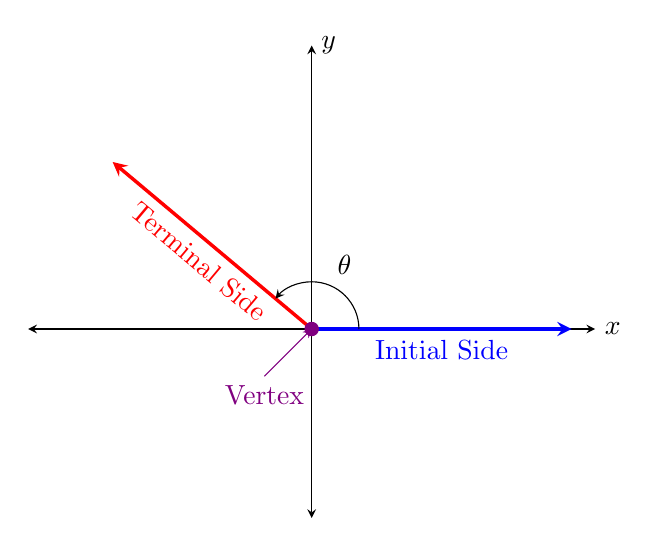
\begin{tikzpicture}[scale=1.2]
    \draw [<->] (-3,0) -- (3,0) node [right] {$x$};
    \draw [<->] (0,-2) -- (0,3) node [right] {$y$};
    \draw [->, >=stealth, line width = 1.25, color=blue] (0,0) -- (2.75,0) node [below, midway] {\color{blue}Initial Side};
    \draw [->, >=stealth, line width = 1.25, color = red] (0,0) -- (140:2.75) node [midway, below, sloped] {\color{red}Terminal Side};
    \draw [color=violet, fill=violet] (0,0) circle (2pt);
    \draw [->, >=stealth, color=violet] (-0.5,-0.5) node [below] {\color{violet}Vertex} -- (0,0); 
    \draw [->, >=stealth] (0:0.5) arc (0:140:0.5) node [midway, above right] {$\theta$};
\end{tikzpicture}
\end{center}
\end{frame}

\begin{frame}{Angles in Standard Position}
    An angle is in \alert{standard position} if    \newline\\  \pause
\begin{itemize}
    \item Vertex is at the origin.  \newline\\  \pause
    \item Initial side runs along positive $x$-axis.    \newline\\  \pause
\end{itemize}

Positive angles open \textbf{counter-clockwise} and negative angles open \textbf{clockwise}.    \newline\\  \pause

A \alert{quadrantal angle} is one whose terminal side lies on an axis. In other words, it's a multiple of $90^\circ$.
\end{frame}


\begin{frame}{Radians}
One \textbf{radian} is the measure of the central angle of a circle in which the radius equals the length of the intercepted arc.    \newline\\

\begin{center}
    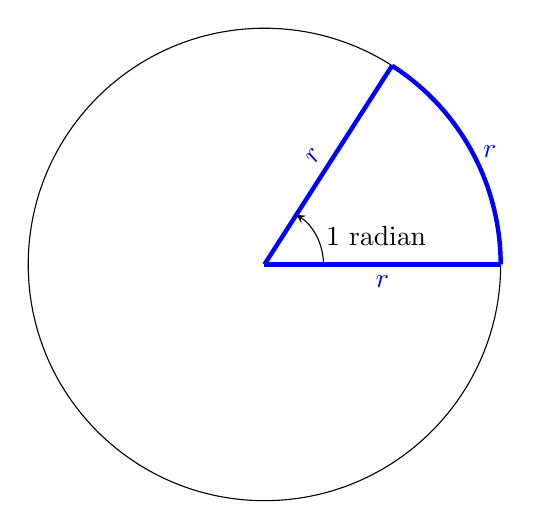
\begin{tikzpicture}
    \draw (0,0) circle (3cm);
    \draw [color = blue, ultra thick] (0,0) -- (3,0) node [below, midway] {$r$};
    \draw [color = blue, ultra thick] (0,0) -- (57.3:3) node [sloped, midway, above] {$r$};
    \draw [line width = 1.5, color = blue, ultra thick] (0:3) arc (0:57.3:3) node [midway, right] {$r$};
    \draw [->, >=stealth] (0:0.75) arc (0:57.3:0.75) node [midway, right] {1 radian};
    \end{tikzpicture}
\end{center}
\end{frame}

\begin{frame}{Radian Interpretation}
In other words, its when the length of your slice of pizza's crust is equal to the radius of the pizza. 
\end{frame}

\section{ Convert degrees to radians and radians to degrees.}

\begin{frame}{Relationship Between Radians and Degrees}
    One rotation is the circumference of the circle ($2\pi r$) and also $360^\circ$:

\begin{align*}
    \onslide<2->{360^\circ &= 2\pi \text{ radians}} \\[10pt]
    \onslide<3->{180^\circ &= \pi \text{ radians} } \\[10pt]
    \onslide<4->{\frac{180^\circ}{\pi} &= \text{1 radian}} \\
\end{align*}
\end{frame}

\begin{frame}{Convert Degrees to Radians and Radians to Degrees}
\begin{itemize}
    \item To convert degrees to radians, multiply by $\frac{\pi}{180^\circ}$.   \\[18pt]  \pause
    \item To convert radians to degrees, multiply by $\frac{180^\circ}{\pi}$.
\end{itemize}
\end{frame}

\begin{frame}{Example 1}
Convert each angle to radians.  \newline\\
(a) \quad $30^\circ$    
\begin{align*}
    \onslide<2->{30^\circ &    }\onslide<3->{\rightarrow30^\circ\left(\frac{\pi}{180^\circ}\right)}   \\[12pt]
    \onslide<4->{&= \frac{30\pi}{180}} \\[12pt]
    \onslide<5->{&= \frac{\pi}{6}}
\end{align*}
\end{frame}

\begin{frame}{Example 1}
Convert each angle to radians.  \newline\\
(b) \quad $90^\circ$    
\begin{align*}
    \onslide<2->{90^\circ &    }\onslide<3->{\rightarrow90^\circ\left(\frac{\pi}{180^\circ}\right)}   \\[12pt]
    \onslide<4->{&= \frac{90\pi}{180}} \\[12pt]
    \onslide<5->{&= \frac{\pi}{2}}
\end{align*}
\end{frame}

\begin{frame}{Example 1}
Convert each angle to radians.  \newline\\
(c) \quad $-135^\circ$    
\begin{align*}
    \onslide<2->{-135^\circ &    }\onslide<3->{\rightarrow-135^\circ\left(\frac{\pi}{180^\circ}\right)}   \\[12pt]
    \onslide<4->{&= \frac{-135\pi}{180}} \\[12pt]
    \onslide<5->{&= \frac{-3\pi}{4}}
\end{align*}
\end{frame}


\begin{frame}{Example 2}
Convert each angle to degrees. \newline\\
(a) \quad $\frac{\pi}{3}$
\begin{align*}
    \onslide<2->{\frac{\pi}{3} &    }\onslide<3->{\rightarrow\frac{\pi}{3}\left(\frac{180^\circ}{\pi}\right)}   \\[12pt]
    \onslide<4->{&= \frac{180^\circ}{3}} \\[12pt]
    \onslide<5->{&= 60^\circ}
\end{align*}
\end{frame}


\begin{frame}{Example 2}
Convert each angle to degrees. \newline\\
(b) \quad $-\frac{5\pi}{4}$
\begin{align*}
    \onslide<2->{-\frac{5\pi}{4} &    }\onslide<3->{\rightarrow-\frac{5\pi}{4}\left(\frac{180^\circ}{\pi}\right)}   \\[12pt]
    \onslide<4->{&= -\frac{900^\circ}{4}} \\[12pt]
    \onslide<5->{&= -225^\circ}
\end{align*}
\end{frame}


\section{ Draw angles in standard position.}

\begin{frame}{Example 3}
Draw and label each angle in standard position. \newline\\
(a) \quad $\alpha = \frac{\pi}{6}$  \qquad \onslide<2->{$\alpha = 30^\circ$}
\begin{center}
\begin{tikzpicture}[scale=1.2]
    \draw [<->] (-2,0) -- (2,0) node [right] {$x$};
    \draw [<->] (0,-2) -- (0,2) node [above] {$y$};
    \draw [->, color=blue, very thick] (0,0) -- (1.5,0);
    \onslide<3->{\draw [->, color=red, very thick] (0,0) -- (30:1.5);}
    \onslide<4->{\draw [->] (0.5,0) arc (0:30:0.5) node [right, yshift=-0.1cm] {$\alpha$};}
\end{tikzpicture}
\end{center}
\end{frame}

\begin{frame}{Example 3}
(b) \quad $\beta = -\frac{4\pi}{3}$ \qquad \onslide<2->{$\beta = -240^\circ$}
\begin{center}
\begin{tikzpicture}[scale=1.2]
    \draw [<->] (-2,0) -- (2,0) node [right] {$x$};
    \draw [<->] (0,-2) -- (0,2) node [above] {$y$};
    \draw [->, color=blue, very thick] (0,0) -- (1.5,0);
    \onslide<3->{\draw [->, color=red, very thick] (0,0) -- (-240:1.5);}
    \onslide<4->{\draw [->] (0.5,0) arc (0:-240:0.5) node [below, xshift=-0.5cm, yshift=-0.75cm] {$\beta$};}
\end{tikzpicture}
\end{center}
\end{frame}

\begin{frame}{Example 3}
(c) \quad   $\gamma = - \frac{9\pi}{4}$ \qquad \onslide<2->{$\gamma = -405^\circ$}
\begin{center}
\begin{tikzpicture}[scale=1.2]
    \draw [<->] (-2,0) -- (2,0) node [right] {$x$};
    \draw [<->] (0,-2) -- (0,2) node [above] {$y$};
    \draw [->, color=blue, very thick] (0,0) -- (1.5,0);
    \onslide<3->{\draw [->, color=red, very thick] (0,0) -- (-405:1.5);}
    \onslide<4->{\bigangle{-405};}
    \onslide<4->{\node at (-0.5,0.5) {$\gamma$};}
\end{tikzpicture}
\end{center}
\end{frame}


\begin{frame}{Example 3}
(d) \quad   $\delta = -\frac{5\pi}{2}$  \qquad \onslide<2->{$\delta = -450^\circ$}
\begin{center}
\begin{tikzpicture}[scale=1.2]
    \draw [<->] (-2,0) -- (2,0) node [right] {$x$};
    \draw [<->] (0,-2) -- (0,2) node [above] {$y$};
    \draw [->, color=blue, very thick] (0,0) -- (1.5,0);
    \onslide<3->{\draw [->, color=red, very thick] (0,0) -- (-450:1.5);}
    \onslide<4->{\bigangle{-450};}
    \onslide<4->{\node at (-0.5,0.5) {$\delta$};}
\end{tikzpicture}
\end{center}
\end{frame}


\section{ Find a coterminal angle to a given angle.}


\begin{frame}{Coterminal Angles}
Two angles that have the same initial and terminal side are \alert{coterminal angles}.    \newline\\  \pause

To find coterminal angles, add (or subtract) multiples of $360^\circ$ (or $2\pi$ radians).
\end{frame}

\begin{frame}{Example 4}
Find a coterminal angle between $0^\circ$ and $360^\circ$ (or 0 and $2\pi$ radians) for each.   \newline\\
(a) \quad   $400^\circ$
\begin{align*}
    \onslide<2->{400^\circ}   
    \onslide<3->{&\rightarrow 400^\circ - 360^\circ} \\[10pt]
    \onslide<4->{&= 40^\circ}
\end{align*}
\end{frame}

\begin{frame}{Example 4}
(b) \quad   $-\frac{4\pi}{3}$
\begin{align*}
    \onslide<2->{-\frac{4\pi}{3}}   
    \onslide<3->{&\rightarrow -\frac{4\pi}{3} + 2\pi} \\[10pt]
    \onslide<4->{&= \frac{2\pi}{3}}
\end{align*}
\end{frame}

\begin{frame}{Example 4}
(c) \quad   $\frac{9\pi}{4}$
\begin{align*}
    \onslide<2->{\frac{9\pi}{4}}   
    \onslide<3->{&\rightarrow \frac{9\pi}{4} - 2\pi} \\[10pt]
    \onslide<4->{&= \frac{\pi}{4}}
\end{align*}
\end{frame}

\begin{frame}{Example 4}
(d) \quad   $-785^\circ$
\begin{align*}
    \onslide<2->{-785^\circ}   
    \onslide<3->{&\rightarrow -785^\circ + 1080^\circ} \\[10pt]
    \onslide<4->{&= 295^\circ}
\end{align*}
\end{frame}

\section{Calculate arc length and sector area}

\begin{frame}{Arc Length}
\begin{center}
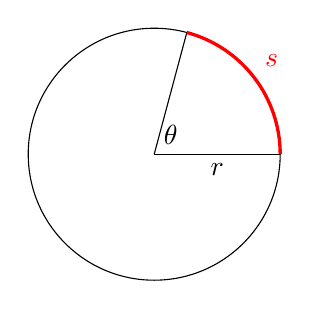
\begin{tikzpicture}[scale=0.8]
    \draw (0,0) circle (2cm);
    \draw (0,0) -- (2,0) node [midway, below] {$r$};
    \draw (0,0) -- (75:2);
    \draw[color=red,very thick] (2,0) arc (0:75:2) node [midway, above right] {$s$};
    \node at (0,0) [above right] {$\theta$};
\end{tikzpicture}
\end{center}
\begin{align*}
    \onslide<2->{\frac{{\color{red}s}}{2\pi r} &= \frac{\theta}{2\pi}}    \\[8pt]
    \onslide<3->{2\pi {\color{red}s} &= 2\pi r \theta} \\[8pt]
    \onslide<4->{{\color{red}s} &= r\theta}
\end{align*}
\end{frame}

\begin{frame}{Sector Area}
\begin{center}
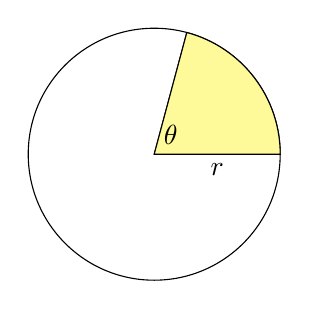
\begin{tikzpicture}[scale=0.8]
    \draw (0,0) circle (2cm);
    \draw (0,0) -- (2,0) node [midway, below] {$r$};
    \draw (0,0) -- (75:2);
    \draw[fill=yellow!40] (0,0) -- (2,0) arc (0:75:2) -- cycle;
    \node at (0,0) [above right] {$\theta$};
\end{tikzpicture}
\end{center}
\begin{align*}
    \onslide<2->{\frac{{\color{blue}A}}{\pi r^2} &= \frac{\theta}{2\pi}}    \\[8pt]
    \onslide<3->{2\pi {\color{blue}A} &= \theta \pi r^2} \\[8pt]
    \onslide<4->{{\color{blue}A} &= \frac{1}{2}\theta r^2 }
\end{align*}
\end{frame}

\begin{frame}{Example 5}
Find the exact arc length and sector area of the circle with \[r = 5\text{ ft}; \, \theta = \frac{\pi}{2}\]    
\onslide<2->{Arc length:}
\begin{align*}
    \onslide<3->{s &= r\theta} \\[6pt]
    \onslide<4->{s &= 5\left(\frac{\pi}{2}\right)} \\[6pt]
    \onslide<5->{s &= \frac{5\pi}{2}\text{ ft}}
\end{align*}
\end{frame}

\begin{frame}{Example 5}
    Sector Area:
\begin{align*}
    \onslide<2->{A &= \frac{1}{2}\theta r^2} \\[12pt]
    \onslide<3->{A &= \frac{1}{2}\left(\frac{\pi}{2}\right)(5^2)} \\[12pt]
    \onslide<4->{A &= \frac{25\pi}{4}\text{ ft\textsuperscript{2}}}
\end{align*}
\end{frame}
    
\end{document}


 